\documentclass[11pt,a4paper]{article}
\usepackage[margin=22mm]{geometry}
\usepackage[T1]{fontenc}
\usepackage{lmodern,amsmath,amssymb,booktabs,array,graphicx,tikz,listings,xcolor,hyperref}
\usetikzlibrary{arrows.meta,positioning,shapes.geometric,calc}
\hypersetup{pdftitle={Cedar-8f2c student reference},pdfauthor={Cedar-8f2c},colorlinks=true,linkcolor=blue,urlcolor=blue}
\lstset{basicstyle=\ttfamily\small,breaklines=true,columns=fullflexible,frame=single}
\newcommand{\bits}[1]{\texttt{#1}}
\newcommand{\reference}{\noindent\textbf{Student reference.} This is an anonymous, editable reconstruction of the supplied student report. It preserves the student's approach and reported results. Editorial verification notes and assignment clarifications are labeled separately. It is not a newly corrected solution or a claim of full fault coverage. The accompanying anonymized PDF preserves the original evidence.\par}
\title{Homework 3: Scan testing and LFSR\\Student reference}
\author{Cedar-8f2c}
\date{}
\begin{document}
\maketitle
\reference

\section{Assignment and supplementary requirements}
The assignment asks for scan insertion into a three-flip-flop finite-state machine, tests for faults $\alpha,\beta,\gamma$, an approach to reduce scan switching without extra hardware overhead, scan-chain organization to reduce testing time, and a modified six-bit LFSR.
The original PDF requests 64 different LFSR patterns. A later supplementary announcement accepts the ordinary 63 nonzero LFSR patterns and counts the reset value as the first pattern. It permits use of a provided testbench, with the enable serving only as a convenient start signal.
A further assignment update explicitly restricts Question 2 to \textbf{two scan paths}, with two scan inputs and two scan outputs.

\section{Question 1(a): The student's scan test}
The student's drawing adds a scan multiplexer in front of each flip-flop. With scan enable asserted, the serial path is
\[
\mathrm{SI}\longrightarrow Q_0\longrightarrow Q_1\longrightarrow Q_2
\longrightarrow\mathrm{SO}.
\]
With scan enable cleared, the flip-flops capture the functional next-state signals.
\begin{figure}[ht]\centering
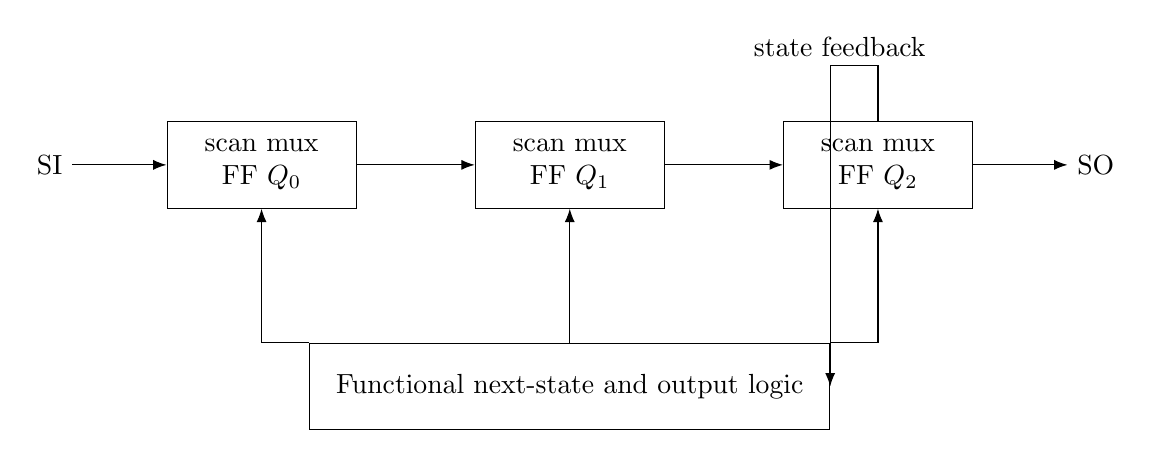
\begin{tikzpicture}[>=Latex,b/.style={draw,align=center,minimum width=24mm,minimum height=11mm}]
\node[b] (q0) {scan mux\\FF $Q_0$};
\node[b,right=15mm of q0] (q1) {scan mux\\FF $Q_1$};
\node[b,right=15mm of q1] (q2) {scan mux\\FF $Q_2$};
\node[b,below=17mm of q1,minimum width=66mm] (comb) {Functional next-state and output logic};
\draw[->](q0)--(q1);\draw[->](q1)--(q2);
\draw[<-](q0.west)--++(-12mm,0)node[left]{SI};
\draw[->](q2.east)--++(12mm,0)node[right]{SO};
\draw[->](comb.north west)-|(q0.south);
\draw[->](comb.north)--(q1.south);
\draw[->](comb.north east)-|(q2.south);
\draw[->](q2.north)--++(0,7mm)-|node[pos=.4,above]{state feedback}(comb.east);
\end{tikzpicture}
\caption{Editable abstraction of the student's scan insertion. The original problem PDF preserves the complete gate-level FSM and marked fault sites.}
\end{figure}
The handwritten report describes the following activation and propagation conditions.
\begin{center}\begin{tabular}{lll}
\toprule Fault & Student's activation & Student's propagation condition\\\midrule
$\alpha$ (SA1)&$\overline{\mathrm{In}}=0$, hence In=1&$Q_0=1$\\
$\beta$ (SA0)&$Q_0=0,\ Q_1=1,\ Q_2=1$&In=1\\
$\gamma$ (SA1)&$\overline{Q_2}=0$, hence $Q_2=1$&$Q_0=0,\ Q_1=1,\ \mathrm{In}=0$\\
\bottomrule\end{tabular}\end{center}
The report's timing explanation is reconstructed below. Clock labels are retained from the handwritten source. An $X$ in the source means a don't-care or arbitrary bit.
\begin{center}\begin{tabular}{p{18mm}>{\raggedright\arraybackslash}p{52mm}>{\raggedright\arraybackslash}p{67mm}}
\toprule Test & Loading and capture & Observation\\\midrule
$\alpha$ & Load SI=1 at clock 2, set In=1, capture at clock 3. & After three shift clocks, inspect SO at clock 6. The source expects zero for the fault-free capture.\\
$\beta$ & Load SI sequence 1,1,0 at clocks 4,5,6, set In=1, capture at clock 7. & Inspect SO after two shifts, at clock 9. The source expects one.\\
$\gamma$ & Load SI sequence 1,1,0 at clocks 8,9,10, set In=0, capture at clock 11. & Observe Out after capture. The source expects zero.\\
\bottomrule\end{tabular}\end{center}
These sequential load and capture steps explain the original two-part timing drawing. The accompanying anonymized PDF retains the complete handwritten waveforms. This reconstruction does not certify the vectors against an independently simulated gate-level FSM.

\section{Question 1(b): The proposed low-switching method}
The student proposes providing an independent scan input and output for each flip-flop, loading all three scan states in parallel. The report's new timing sketch uses alternating parallel-load and capture operations for the three fault tests. For $\alpha$, it loads $Q_0=1$ and uses In=1. For $\beta$, it loads $(Q_2,Q_1,Q_0)=(1,1,0)$ and uses In=1. For $\gamma$, it loads the same state and uses In=0.
\paragraph{Grading feedback.}
The supplied feedback explicitly says this approach adds hardware overhead. Extra scan inputs and outputs do not satisfy the question's constraint. The proposal is preserved as a student reference, rather than presented as an acceptable solution.

\section{Question 2: The student's original time calculations}
The blocks contain the following scan flip-flops and pattern requirements:
\begin{center}\begin{tabular}{lrr}
\toprule Block&Scan flip-flops&Patterns\\\midrule
1&200&300\\2&300&80\\3&500&700\\\bottomrule
\end{tabular}\end{center}
For part (a), the student puts blocks 1 and 2 on one serial path, and block 3 on the other. The submitted calculation adds the pattern requirements:
\begin{align*}
T_{1+2}^{\rm student}&=(300+80+1)(200+300)+300+80=190880,\\
T_3^{\rm student}&=(700+1)500+700=351200.
\end{align*}
The report therefore claims a minimum of $351200$ clock periods.
\paragraph{Grading feedback.}
For serially concatenated blocks that are tested in parallel by each combined vector, the pattern count is $\max(300,80)=300$, rather than $300+80$. The supplied feedback gives
\[
T_{1+2}=(300+1)(200+300)+300=150800.
\]
The student's numerical expression for this path is incorrect even though block 3 can still dominate the schedule.

For part (b), block 3 is split into a 300-flip-flop block and a 200-flip-flop block, each requiring 400 patterns. The report groups block 1 with the 200-flip-flop piece and block 2 with the 300-flip-flop piece. It calculates
\begin{align*}
T_{\rm left}^{\rm student}&=(300+400+1)(200+200)+300+400=281100,\\
T_{\rm right}^{\rm student}&=(80+400+1)(300+300)+80+400=289080.
\end{align*}
The student claims a minimum of $289080$ periods.
\paragraph{Grading feedback.}
The same pattern-count error applies. With this proposed grouping, using the feedback's convention gives
\[
T_{\rm left}=(400+1)400+400=160800,\qquad
T_{\rm right}=(400+1)600+400=241000.
\]
These values correct the arithmetic for the student's grouping only. They do not establish that this grouping is globally optimal under the two-path constraint.

\section{Question 3: The retained six-bit LFSR}
The student draws a six-stage LFSR with feedback from the final two stages. The Verilog uses the following recurrence:
\[
Q_0^+=Q_4\oplus Q_5,\qquad Q_i^+=Q_{i-1}\quad(1\le i\le5).
\]
The active-low reset initializes the state to 000001. When enable is low, the state holds.
\begin{figure}[ht]\centering
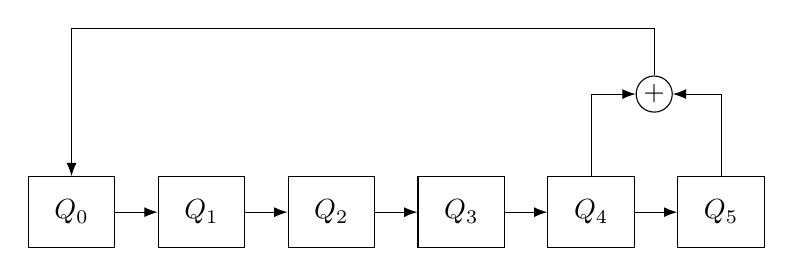
\begin{tikzpicture}[>=Latex,b/.style={draw,minimum width=11mm,minimum height=9mm}]
\foreach \i in {0,...,5}{\node[b] (q\i) at (\i*1.65,0) {$Q_\i$};}
\foreach \i/\j in {0/1,1/2,2/3,3/4,4/5}{\draw[->](q\i)--(q\j);}
\node[draw,circle,inner sep=1pt] (xor) at (7.4,1.5) {$+$};
\draw[->](q4.north)|-(xor.west);
\draw[->](q5.north)|-(xor.east);
\draw[->](xor.north)--++(0,6mm)-|(q0.north);
\end{tikzpicture}
\caption{Editable reconstruction of the six-bit LFSR diagram.}
\end{figure}
The supplied testbench accumulates 63 output values and declares pass if their sum is 2016:
\[
1+2+\cdots+63=2016.
\]
The original report shows the \bits{PASS} signal high.
\paragraph{Editorial verification notes.}
The sum alone cannot prove uniqueness, since repeated values can have the same total. A stronger check should track each of the 64 possible states and verify the expected period.
The retained recurrence never reaches the all-zero state from its nonzero seed, so it can generate 63 states, not the original PDF's 64-state exhaustive sequence. This matches the later supplementary announcement, but it is not a modified exhaustive 64-state generator.

\section{Source selection and evidence}
The submitted \bits{LFSR.v} and \bits{LFSR\_tb.v} form the complete source set. The project source named \bits{HW3.v} is identical to \bits{LFSR.v}, so that duplicate is unnecessary. The original report has six pages, including two assignment pages and one blank page. Its anonymous PDF preserves the original page count. The original supplementary screenshots and grading interface are not republished because they contain identities. Their technical requirements and relevant feedback are transcribed above.
\section{Repository verification}
Icarus Verilog 13.0 executes the original testbench and prints PASS. An independent testbench uses a 64-bit seen-state set instead of relying on the sum alone. It observes 63 unique nonzero states, no duplicates during the 63-state traversal, sum 2016, no all-zero state, and a return to seed 000001 after 63 enabled transitions. This establishes the stated nonzero period for this implementation. The handwritten scan-test vectors have not been independently simulated against a reconstructed gate-level FSM, and the original proposed scan-power method retains the grading objection above.
\end{document}
